\chapter{Numerical experiments}
\label{cha:numer-experiments}

In this section we apply the complete FEM/BEM scheme with adaptive IMR and nodal integration, as developed in \crefs{sec:galerk-meth-llg, sec:hybr-finit-elem, sec:adaptive-imr}, to ``real-world'' micromagnetics problems.

The ??ds-th problem solved is a case where an exact solution exists.

The ??ds-th problem we tackle is the \mumag standard problem 4 \cite{mumag-website}, which is widely used to test dynamic micromagnetic codes.



\section{??ds solution}
\label{sec:numer-exper}


\subsection{Problem definition}

We solve the LLG without magnetostatics on a two dimensional square domain with periodic boundary conditions.

In the following experiments we use the wave exact solution in 2D (see \cref{sec:wave-like-solution}) for simplicity and because an exact solution is known.
The solution parameters used are $\kvec = 2\pi$ so that the solution is periodic on domains of unit size and $c = 0.35\pi$ which gives large amplitude oscillations without while still remaining in the wave-like parameter regime.



This problem allows us to test the convergence and conservation properties of IMR + FEM + nodal quadrature.
In particular the existence of an exact solution for the LLG with exchange is key for the convergence experiments.
Unfortunately we do not know of any non-trivial (\ie with $\mv$ varying in both space and time) exact solution for the LLG with exchange and magnetostatics.
  

\subsection{Implementation}

FEM

No magnetostatics so there is no for the FEM/BEM method

nodal and Gaussian quadrature

IMR

Newton-Raphson, the newton tolerance is ??ds.
The Newton tolerance is set to $10^{-14}$ unless otherwise specified.

The linear systems are solved using GMRES with an ILU-1 preconditioner\footnote{Hypre, parameters: ??ds}. 
The GMRES tolerance is set to ??ds



\subsection{Accuracy of nodal quadrature}



\subsection{Convergence}

Since we have an exact solution for this example we can calculate the total error and plot the convergence as $\dtn \goesto 0$ and $h \goesto 0$.
Following the example of Jeong \etal \cite{Jeong2014} we link the spatial discretisation length to the time step by $\dtn = 0.32h$.

We plot two figures: convergence of a single step and convergence after some time.

??ds


\subsection{Magnetisation length conservation}

First we examine the evolution of the magnetisation length error over time in a single case.
We used $\dampc = 0.001$, a mesh of square elements with $6561$ nodes and constant time step sizes of $\dtn = 0.001$. 
These choices of mesh and time step resolve the solution well, as can be seen in the convergence experiments above.
The maximum time was $t_{max} = 5$ ($\approx 20$ wave periods), the damping is small enough that the oscillations continue well past this time. % trace in folder ??ds check it
\cref{fig:mean-ml-error-2d-gauss} shows the behaviour of the maximum (over all nodes) error in magnetisation length, \cref{fig:mean-ml-error-2d-nodal} shows the equivalent plot when using nodal quadrature.
When using nodal quadrature the error never grows much larger than the Newton tolerance, whereas when using Gaussian quadrature the error grows to $\order{10^{-5}}$ within the short simultation.

\begin{figure}
  \centering
  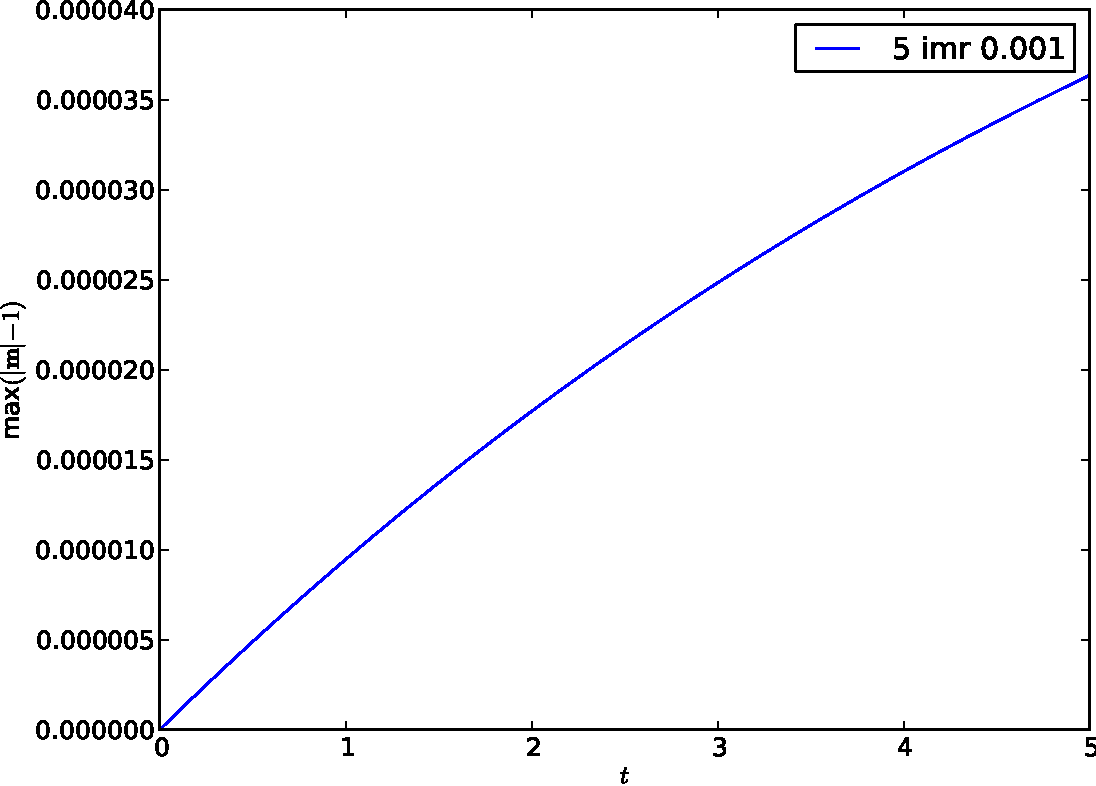
\includegraphics[width=0.8\textwidth]{plots/2d_wave_solution_m_length/gauss-maxmathbfm-1vst.pdf}
  \caption{Evolution of the maximum error of nodal magnetisation lengths in the 2D wave example with a standard Gaussian quadrature scheme.}
  \label{fig:mean-ml-error-2d-gauss}
\end{figure}

\begin{figure}
  \centering
  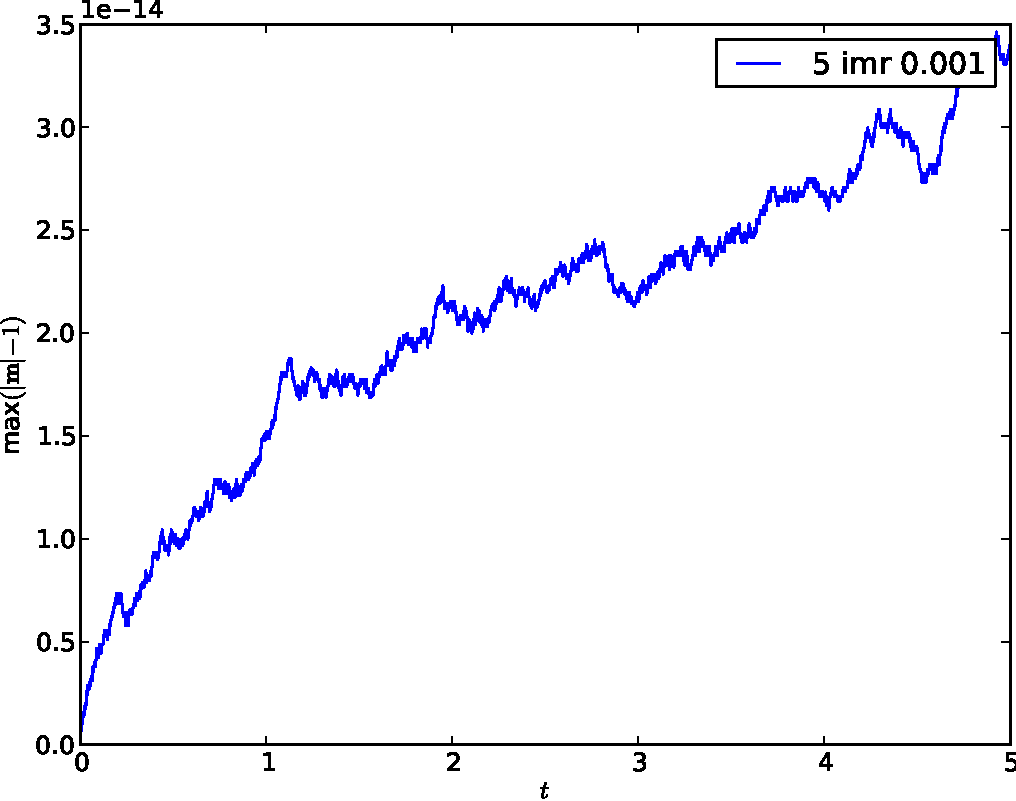
\includegraphics[width=0.8\textwidth]{plots/2d_wave_solution_m_length/lnodal-maxmathbfm-1vst.pdf}
  \caption{Evolution of the maximum error of nodal magnetisation lengths in the 2D wave example with the nodal quadrature scheme introduced above.}
  \label{fig:mean-ml-error-2d-nodal}
\end{figure}

To check that the conservation is independent of problem parameters we ran a parameter sweep using: square and triangle elements; 36, 441 and 6561 nodes; time steps of $0.1$, $0.01$ and $0.001$; and damping parameters of $1$, $0.1$, $0.001$ and $0$.
The maximum length error over all parameter sets, all time steps and all nodes when using nodal quadrature was 2.364775e-12, when using Gaussian quadrature it was 0.013746647.
This clearly demonstrates the necessity and effectiveness of the nodal quadrature scheme for retaining the conservation properties of the implicit midpoint rule.
% using the same data as for the figures above, look in their folders for parameter sets data parsing command: parse.py -d /mnt/moredata/optoomph/user_drivers/micromagnetics/experiments/parameter_sweeps/parameter_file_0/ -l=-dt -l=-damping --split=-integration --print-data max-max-ml --print-data ml -l=initial_nnode


??ds describe very long time behaviour in \cref{fig:mean-ml-error-2d-nodal-long-time}.

\begin{figure}
  \centering
  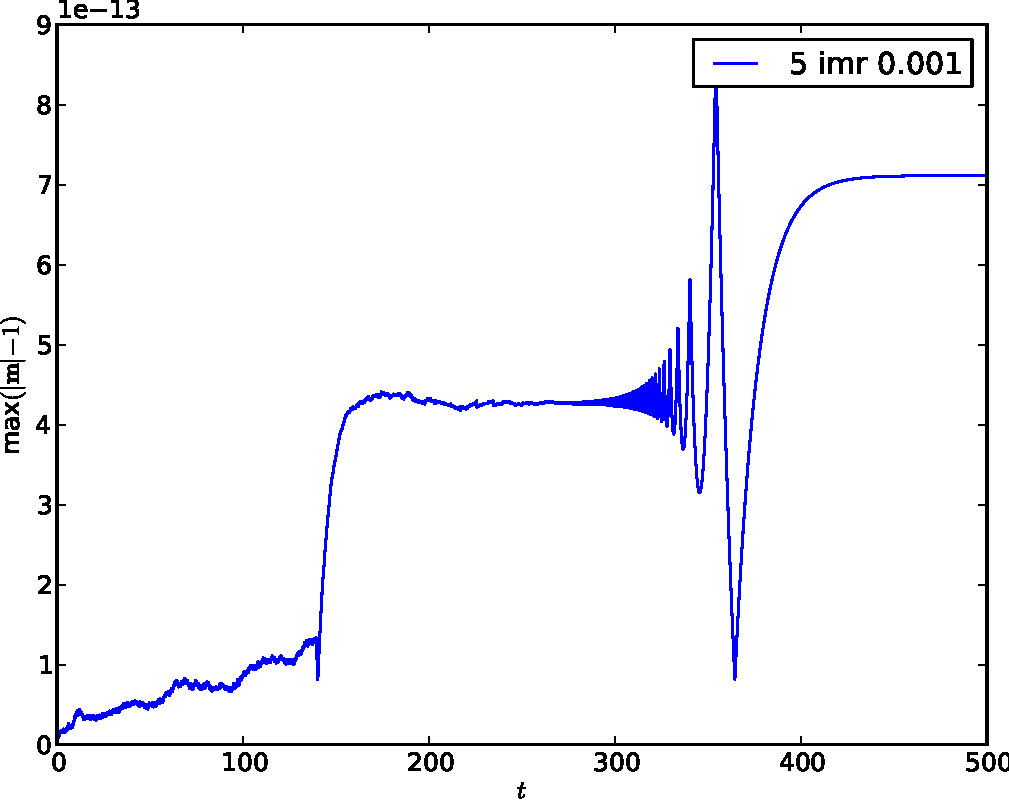
\includegraphics[width=0.8\textwidth]{plots/2d_wave_solution_m_length_long_time/-maxmathbfm-1vst.pdf}
  \caption{Evolution of the maximum error of nodal magnetisation lengths in the 2D wave example with the nodal quadrature scheme over a very long time period.}
  \label{fig:mean-ml-error-2d-nodal-long-time}
\end{figure}



\subsection{Effect of Newton tolerance}
\label{sec:effect-newt-toler-m-conservation}

Since the non-linear residual \cref{eq:weak-llg} used in the derivation of the conservation properties is only true up to the accuracy of the linearisation method we would expect to see some effect when modifying this accuracy.
In our model Newton's method is used for linearisation (see \cref{sec:newt-raph})so the relevant measure of accuracy is the Newton tolerance.

The obvious experiment to carry out would be to vary the Newton tolerance and examine how the error in $\abs{\mv}$ is affected.
However Newton's method extremely quickly meaning that the final residual is sometimes orders of magnitude smaller than the tolerance, this would hide any corrolation between the tolerance and the error.
Instead we plot the error against the actual maximum residual obtained (specifically: the mean over time steps of $\norm{\rv}_\infty$ after the Newton method has converged). 
The results are shown in \cref{fig:mean-ml-error-2d-nodal-newton-tests}, there is a clear corrolation between small residuals and small length errors.


\begin{figure}
  \centering
  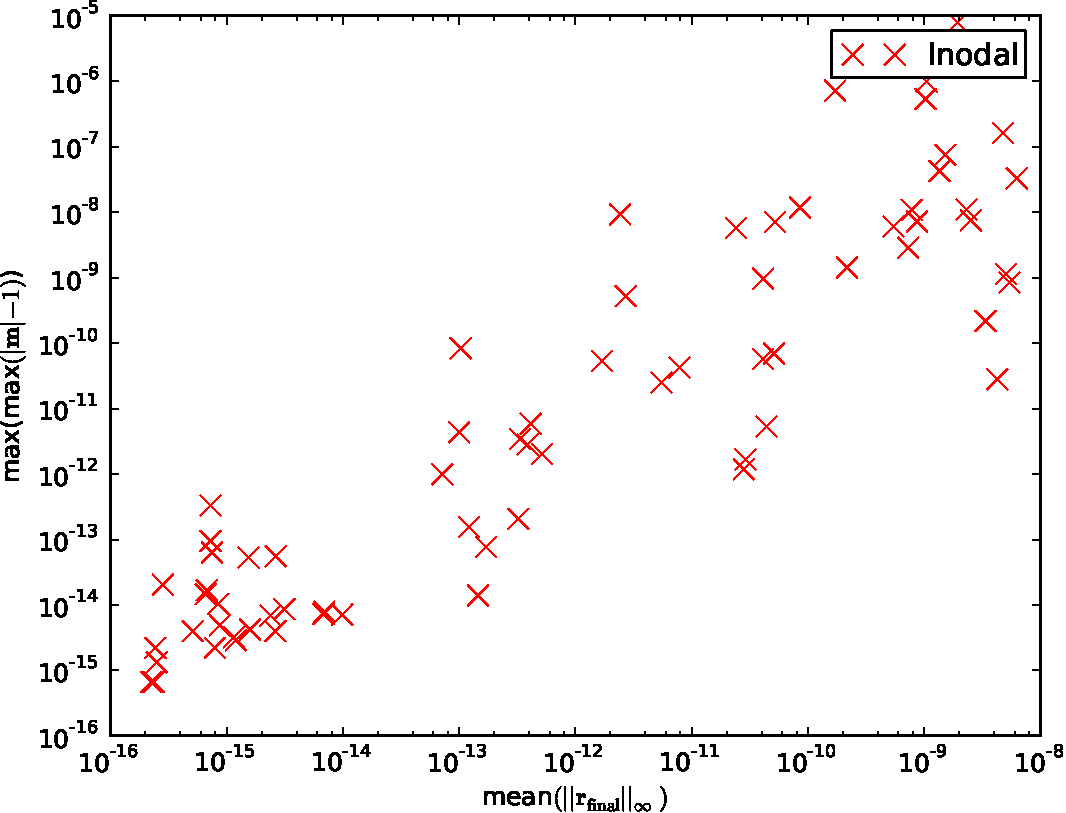
\includegraphics[width=0.8\textwidth]
  {plots/2d_wave_solution_m_length_newton_res/-maxmaxmathbfm-1vsmeanmathbfr_mathrmfinal_infty.pdf}
  \caption{Corrolation between maximum error of nodal magnetisation lengths and largest maximum Newton residual after convergence in the 2D wave example with the nodal quadrature scheme over a very long time period.}
  \label{fig:mean-ml-error-2d-nodal-newton-tests}
\end{figure}


% \subsection{Adaptivity}
% ??ds - no need for this? leave it to the final subsection?

% It remains to demonstrate that the adaptivity scheme introduced in \cref{sec:adaptive-imr} is effective for the finite element problem with nodal integration.
% Since there is still no relationship with previous time step sizes in the conservation proofs with nodal integration we don't expect there to be any issues with variable step size and conservation.

% Additionally our discretisation can be written as semi-discretisation in space (giving a system of ODEs) followed by the application of IMR in time.
% Hence we have no reason to expect the adaptive IMR to behave any differently to in the pure ODE case.

% \subsection{BEM}
% ??ds - no need for this? leave it to the final subsection?


% ??ds

\subsection{Conclusions}



\section{The \mumag standard problem 4}

Widely used to test micromagnetic codes

Reversal of a thin film of permalloy under two different fields

Unfortunately FEM/BEM magnetostatic calcultations are extremely unsuited to thin film problems (the dense BEM matrix size is proportional to the size of the boundary, in thin films the entire problem is on the boundary. The additional geometric flexibility is not needed for simple cubeoid shapes.)
But we will do it anyway in order to test our results.


\subsection{Problem specification}

The problem specification is as follows:

The magnetic domain is a simple sheet of magnetic material $500 \times 125 \times 3$nm with material parameters
\begin{equation}
  \begin{aligned}
    A &= 1.3\E{-11} \text{J/m}, \\
    M_s &= 8.0\E{5} \text{A/m}, \\
    \Kone &= 0.0, \\
    \gymagc &= 2.211 \E{5} \text{m/As}, \\
    \dampc &= 0.02.
  \end{aligned}
\end{equation}
Two different applied fields should be used, correspond to two different solutions:
\begin{equation}
  \begin{aligned}
    \happ_1 = [-24.6, 4.3, 0.0] \E{-3}\text{A/m}, \\
    \happ_1 = [-35.5, -6.3, 0.0] \E{-3}\text{A/m}, \\
  \end{aligned}
  \label{eq:mumag-h-app}
\end{equation}
where we have converted from the magnetic flux intensity specified by the \mumag website to magnetic field by dropping a factor of $\mu_0$ from the RHS.
The initial condition is the result of relaxing the magnetisation from the state created by a saturating field in the $[1,1,1]$.

The magnetic parameters result in a magnetostatic exchange length (and simulation unit length) of
\begin{equation}
  l_{\text{ex}} = \sqrt{\frac{2A}{\mu_0 M_s^2}} = 5.6858\text{nm},
\end{equation}
hence the normalised dimensions are $500 \times 125 \times 3 / 5.6858$.
The unit time is
\begin{equation}
  t_{\text{unit}} = \frac{1}{\gymagc M_s} = 5.653\text{ps}.
\end{equation}
The normalised applied fields are simply the fields given in \cref{eq:mumag-h-app} divided by $M_s = 8.0\E{5}$.

\subsection{Numerical methods and parameters}

Mesh

Newton tol

quadrature(s)

time integrator(s)

solvers

etc.


\subsection{Results}

Plot dynamics with some other peoples.

Conservation properties of IMR.


\section{Reversal of a magnetic nanotube?}

More relevant problem for FEM/BEM methods--non-trivial geometry.

More relevant for conservation properties: complex, long time dynamics.


\subsection{Problem specification}

??ds


\subsection{Numerical methods and parameters}

??ds mesh generation



\subsection{Results}

??ds convergence: space and time


??ds conservation: m and energy


??ds adaptivity


??ds comparison to other methods?


%%% Local Variables:
%%% mode: latex
%%% TeX-master: "main"
%%% End:
